\section{Topologies for real-time multimedia communication}
\label{sec:topologies}

%% 
%% Leave first page empty
\thispagestyle{empty}

In this chapter we discuss different possible topologies that can be used in real time media communication.

A topology is defined as the arrangement of the various nodes of a network together. Nodes can be connected through different links and configurations. 

Network topologies are determined by network protocols as opposed to by physical cables, wires or devices. We can think of a topology as a virtual network shape or structure. This shape does not usually match the physical layout but focuses on the logical map of the network. For example, computers in a building can be arranged physically in a circle, but it would be highly unlikely to find them defined as a ring topology.

Topologies are composed by multiple devices used to extend cable connections, concentrate interfaces, convert data formats and security. Commonly, routers are used to concentrate multiple connections and provide connectivity to a Wide Area Network \nomenclature{Wide Area Network}{WAN}. They have the responsibility of routing data packets from the source to the destination within the Local Area Network \nomenclature{Local Area Network}{LAN} or WAN.  

However, routers may also occur to provide some issues as they usually activate security mechanisms that affect WebRTC. For example, NAT traversal problems decide either if the call is established or not, this problem can be solved in WebRTC with the usage of TURN and STUN, described in Section~\ref{sec:internals}. However, in some restrictive environments it might be impossible to succeed with the call establishment. 

The usage of NAT traversal mechanisms in WebRTC is crucial and at the same time increases the complexity of the browser internals (Section~\ref{sec:internals}). STUN and TURN servers must be reachable from the browser in order to provide the best {\it candidates} that are evaluated by the ICE mechanism.

All the mentioned mechanisms provide high level of success but might fail in very restrictive environments. To solve some of the issues, WebRTC allows UDP and TCP (using TURN) packet transport, this is done in order to enable connectivity even in very restrictive environments that may have UDP packet drop mechanisms. 

For some topologies that include the establishment of multiple {\it PeerConnections}, resource usage can be a big problem (e.g. mesh, one-to-many or tree). Considering that system capacity relies on how the OS architecture handles processes, CPU and memory usage of WebRTC might be seen as a constraint for those topologies. For example, in Unix based systems every tab of a browser is treated as a separate process meanwhile in other architectures this might be handled differently. Media encoding usually consume most of those resources becoming a bottleneck for some scenarios.

In this section we describe the following topologies for WebRTC: Point-to-point, one-to-many, many-to-many, usage of MCU and overlay networks. Those are some of the most common used topologies. However, some of them are still not possible to implement with the current WebRTC API.

\subsection{Point-to-Point}

The simplest topology is a communication between two nodes or endpoints. This model is widely used in telephony and provides simple real time communication between users. In WebRTC, point-to-point topologies work only within people in the same domain in contrast to cross-domain communication alternatives such as SIP. Scenarios such as the one shown in Figure~\ref{fig:SIParchitecture} are difficult to design in a WebRTC application, on the other side, Figure~\ref{fig:webrtcExample} presents the most common WebRTC point-to-point scenario.

There can be two different types of ponit-to-point topologies: dedicated or switched. Dedicated topologies appears to the user as a permanently associated communication channel between two endpoints. Within many switched telecommunications system it is possible to establish a permanent circuit. The resources in such connection can be released when no longer needed.

On the other side, switched networks are the most common network topology for WebRTC. It is defined as a point-to-point circuit that can be set up a dynamic path thanks to packet-switching technologies and dropped when no longer needed. 

Uses for point-to-point topologies in real-time communications are usually related to bidirectional communications between two endpoints. Other uses can also be given in data transmission between devices. Traditional radio links also rely on point-to-point topologies.
 
\subsection{One-to-Many}

One-to-many or star topologies are one of the most common network topologies for synchronous and asynchronous media streaming (e.g Windows Media Server or RTMFP). This kind of topology consists of a central node that transmits streams to the rest of nodes connected to it. In the WebRTC example of Figure~\ref{fig:starExample}, the central node might be also receiving real time data in difference of the traditional streaming scenarios providing P2P communication between the peers and the central node.

 \begin{figure}[h]
  \centering
    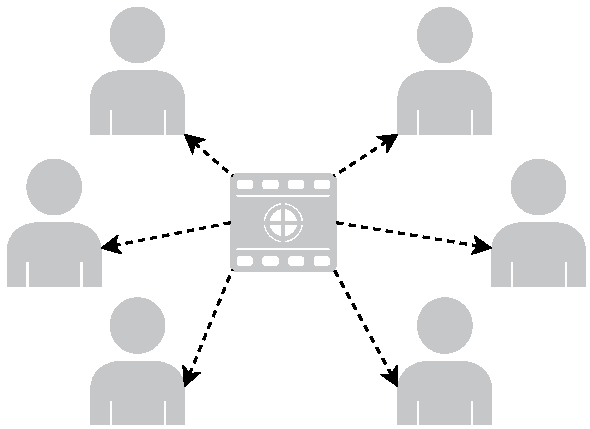
\includegraphics[width=0.5\textwidth]{./figures/star.pdf}
      \caption[Multi-unicast topology for real time media]{Multi-unicast topology for real time media.}
	\label{fig:starExample}
\end{figure}

This central node provides a connection point for all nodes. This type of topology reduces the change of network failure by connecting all the clients to a central device. When this happens each client can fail individually without affecting the rest of the network. However, this might also produce high dependency on the central node. If this node fails, all the connectivity is lost. All the peripheral nodes may communicate with all others by transmitting to, and receiving from, the central device. This behavior can be given when using rebroadcasting.

One-to-many topologies can provide some advantages. Better performance, as the packets are not processed by an excessive number of nodes before being delivered. Resiliency against endpoint failures, this isolation also prevents non-centralized failure from affecting the rest of nodes. Start topologies also make it easier to detect and localize faulty nodes. Furthermore, there are no disruptions when adding or removing endpoints on the network.

On the other hand, this topology relies on high dependence of the central node that sends the traffic. If this node fails, the network becomes inoperable. The central node will also act as a bottleneck, calculating its capacity is required when seizing the network.

In a WebRTC star topology we have a video, audio and data provided from one source to multiple endpoints. This might cause a huge load on the source when having multiple {\it PeerConnection} running, central node bottleneck behavior can be a constraint in this scenario. Compared with other topologies, media delay on the network is not a good indicator for this topology due to the one-way communication only. In some scenarios we may not require data to be received on the source. Those scenarios are one-way only use cases.

Common uses for star scenarios are related with video and audio streaming to multiple peers, TV media and conferencing. Live streaming is a common use for internet TV. For example, media providers could use this topology when sending media streams from the source to multiple endpoints. This could allow their subscribers to join any channel when desired. 

Other WebRTC solutions could cover communication betweeen employees with an HMTL5 web application. Music bands also could take advantage of this scenario by being able to transmit their show to the audience with feedback in real time or having the members playing from different geographic areas. All the previous examples take advantage of WebRTC by having direct feedback from the connected nodes, current media streaming technologies do not provide this kind of communication between the viewer and the origin.

\subsection{Many-to-Many}

Many-to-many topologies are also known as full mesh. In this type of topology, each network node is interconnected with every other node. Each endpoint sends and receives data from each other node of the network.

In a full mesh topology all peers connect between themselves increasing the number of connections and used resources. The value of fully meshed networks depend on the number of subscribers, the number of {\it PeerConnections} established in a mesh network is dependent on the amount of people in the conference. The number of {\it PeerConnections} in a full mesh topology can grow rapidly proportionally to the square of amount of the nodes.

Full mesh topologies provide some advantages. They can expand and be modified without disrupting other nodes. Furthermore, data can be transmitted from different devices simultaneously. On the other hand, the overall cost of this network is high compared with other topologies. Maintenance of this topology is also very difficult and traffic load is high.

This topology is used in wireless and backbone networks. WebRTC uses are related to video conferencing. Conferencing systems are widely extended in enterprises for long-distance communication between employees and working groups. It can also be used to transfer data between peers as a file delivery network. 

%Equation~\ref{eq:meshformula}
%\begin{equation}
%	\label{eq:meshformula}
%	c = \frac{n(n-1)}{2}\\
%	
%	c \text{: Number of {\it PeerConnections}}\
%		
%	n \text{: Nodes in the mesh}
%\end{equation}
%
%Equation~\ref{eq:meshformula} calculates the amount of WebRTC connections required for a {\it full mesh} topology. 

\subsection{Multipoint Conferencing Unit (MCU)}

Multipoint Conferencing Unit (MCU) \nomenclature{MCU}{Multipoint Conferencing Unit} is a device used to bridge streams in conferences, it multiplexes, mixes and encodes media of different sources to be sent over one gateway. MCU usage could be a good alternative when designing WebRTC video conferencing applications. %the ability to multiplex different streams into the same channel is going to directly affect on how the client performs when reproducing the video.

In real time media topologies, MCU is a common component, used as relay it helps end devices to handle less load for the sources by multiplexing all the streams of the call into the same channel, we can have multiple peers connected to the same MCU that can multiplex the media sent by all of them into one unique stream forwarded to all the participants of the call.

MCUs receive the streams from the clients and multiplex them over one unique channel, this provides good scalability from the client perspective because it is only building one connection even though there are multiple peers on the conference.

Some MCUs may have to encode and decode media on the fly, this can be difficult in real time applications but can provide different encoding options to adapt the stream output to the link conditions. 

Drawbacks of the MCU model are related to the dependency of the end nodes on the MCU, if the MCU fails to give good latency and performance, the call quality is affected and receivers do not get the expected response. Load in the MCU depend on the number of participants per conference and the number of conferences going through the MCU. A scalable implementation is needed when handling multiple conferences. A different alternative is the usage of cascaded MCUs to provide more scalability.  

\subsection{Overlay}

Overlaying media streams is the ability of a peer to forward data to a third party. Systems that implement overlay are those that require the media to be forwarded from one peer to the other. Multiple topologies can be constructed using overlaying. Some examples are {\it hub-spoke} or {\it tree}, seen in Figure~\ref{fig:overlaytopologies}.

We can combine all of the following topologies to build an infrastructure that fits our requirements. 

In WebRTC we can use overlay to forward media streams from one node to another. This feature can be very useful when building scalable applications. We can design multiple layers of nodes that transmit the media relaying to each other. Other alternatives would be the usage of overlaying in mesh or one-to-many topologies. In those environments, nodes could forward the stream to provide reliability on the network. However, WebRTC does not provide native support for media overlay yet, but it is planned to implement those features in future versions of the API.

Overlay scenarios have some disadvantages. Topologies that rely on this technique usually are slow distributing the data, this produces long latency. Furthermore, overlay can also provide duplicate packets at certain points.

Overlaying is widely used in audio and video conferencing, multi-party games and content distribution protocols. Considering WebRTC it could also be implemented in group communication applications. 
 
\begin{figure}[h]
        \centering
        \begin{subfigure}[b]{0.5\textwidth}
                \centering
                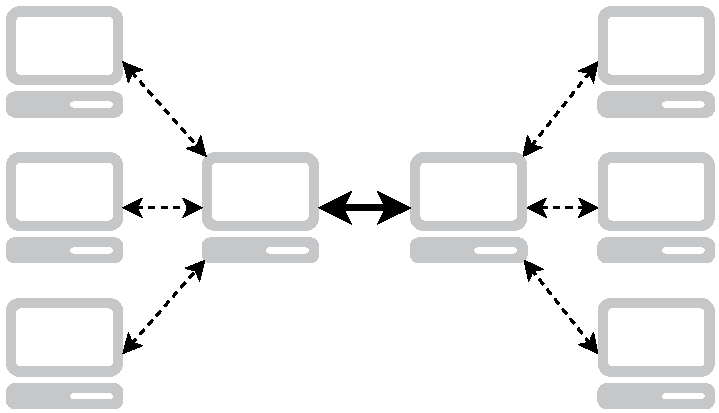
\includegraphics[width=\textwidth]{./figures/hubandspoke.pdf}
                \caption{Hub-spoke topology}
                \label{fig:hubandspoke}
        \end{subfigure}%
        ~ %add desired spacing between images, e. g. ~, \quad, \qquad etc.
          %(or a blank line to force the subfigure onto a new line)
        \begin{subfigure}[b]{0.5\textwidth}
                \centering
                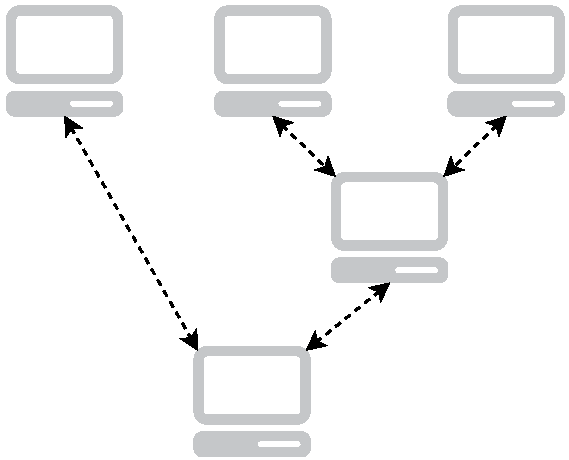
\includegraphics[width=\textwidth]{./figures/three.pdf}
                \caption{Tree topology}
                \label{fig:three}
        \end{subfigure}
        \caption[Overlay topologies]{Overlay topologies.}
        \label{fig:overlaytopologies}
\end{figure}

\subsubsection{Hub-spoke}

Hub-spoke distribution is a topology composed of multiple nodes and arranged like a chariot wheel. Traffic flows along spokes that are connected to the hub at the center. This type of topology, represented in Figure~\ref{fig:hubandspoke}, behaves well in some scenarios as it requires less connections to perform a full communication in the network. 

On this type of topology, hubs are designed to forward traffic from one node to another. However, those devices are not always dedicated machines. In some specific protocols it is possible that hubs are common endpoint devices selected to act as dynamic hubs. For example, in Skype, user computers can act as hubs forwarding calls to other nodes. This happens when the response of those devices is very good, then the protocol selects the best candidate and triggers it to operate as a hub in the network. From then this endpoint becomes a node that forwards data to other peers. 

Hub-spoke model has some advantages. The amount of paths to connect all nodes is significantly less than other topologies. Having less amount of paths also makes the topology to be more efficient in terms of resources. Lastly, new spokes can be created easily without affecting the rest of nodes in the network much.

However, due to a centralized hub model, the reliability of the network is based on this central node. Previous statements of dynamic hubs can help to reduce the dependency of central nodes. Resources have to be seized optimally to avoid overload of the hub.

\subsubsection{Tree}
 
Tree topology is based on a node hierarchy, the highest level of the tree consists of a single node that is connected to one or more nodes that forward the traffic to the other layers of the topology. Tree topologies are not constrained by the number of levels and can adapt to the required number of end users as seen in Figure~\ref{fig:three}.  

This type of topologies are scalable and manageable. In case of failure it is relatively easy to identify the broken branch of the tree and repair that node. The expansion of this type of network is easy.

On the other hand, we can have connectivity problems if a node fails to keep the link up, all the layers under that node are going to be affected and the media forwarding will stop. Overlay is crucial for this topology that is widely used in media streaming, for real time communications. Large tree topologies won't be the best candidates given the delay produced when forwarding the packets from different layers.

Topologies such as tree are not only used for media streaming but they can also be used to provide wireless coverage in difficult areas, acting as hotspots, each hop can extend the coverage of the wireless in remote areas.

\subsection{Summary of topologies}

Different topologies can be used for real-time communication. This section has described the ones that can adapt to WebRTC in different use cases. However, some of them are still not possible to implement due to technology constraints. 

During this thesis we focus our study in point-to-point, many-to-many and MCU topologies. Those two topologies can adapt to WebRTC application requirements. 